
\chapter{Valid Outcomes of Positive Support Size Four}

We want to show that for all valid integral outcomes \( \mathbf w \) with \( |\mathrm{supp}^+(\mathbf w)| = 4 \) we have
\begin{align*}
    \mathrm{deg}(\mathbf w) \leq 2 \cdot |\mathrm{supp}^+(\mathbf w)| - 3 = 5.
\end{align*}
In the previous chapter, we showed that this inequality holds for all valid integral outcomes \( \mathbf w \) with \( |\mathrm{supp}^+(\mathbf w)| \leq 3 \) using the \emph{Invertibility Criterion}. For this chapter, we will need to introduce a new criterion, the \emph{Hyperfield Criterion}.

\section{Hyperfield Criterion}

Let us define the {sign hyperfield}. For some set \( A \), the set \( 2^A \) denotes the power set of \( A \).

\begin{definition}
    Let \( H \coloneqq \left\{ -1, 0, 1 \right\} \). We define the addition \( + : H \times H \to 2^H \setminus \left\{ \emptyset \right\} \) on \( H \) as follows
    \begin{align*}
        0 + x = \left\{ x \right\}  \quad \forall x \in H, \quad 1 + 1 = \left\{ 1 \right\}, \quad 1 + (-1) = H, \quad (-1) + (-1) = \left\{ -1 \right\}.
    \end{align*}
    Multiplication \( \times : H \times H \to H \) is defined as usual. We call \( H \) the \emph{sign hyperfield}.
\end{definition}

Often, for singleton sets \( \left\{ x \right\} \), we will write \( x \) instead of \( \left\{ x \right\} \). So, 
\begin{align*}
    1 + 1 = 1 \qquad \qquad \text{or} \qquad \qquad (-1) + 0 = -1.
\end{align*}

\begin{remark}
    The tuple \( (H, + , \cdot, 0, 1) \) is called a \emph{hyperfield}. A hyperfield satisfies the following properties:
    \begin{enumerate}
        \item  The maps \( + \) and \( \cdot \) are symmetric;
        \item \( (H \setminus \left\{ 0 \right\}, \cdot, 1) \) is a group;
        \item \( 0 \cdot x = 0 \) and \( 0 + x = x \) hold for all \( x \in H \);
        \item \( \bigcup_{q \in x+y}(q + z) = \bigcup_{q \in x + y}(x + q) \) hold for all \( x,y,z \in H \);
        \item \( a \cdot (x + y) = (a \cdot x) + (a \cdot y) \) hold for all \( a,x,y \in H \).
        \item An inverse element \( y  \in H\) exists for every \( x \in H\) such that the set \( x + y \) contains \( 0 \). This inverse element \( y \) is unique for every \( x \) and is denoted by \( -x \).
    \end{enumerate}

    Refer to \cite{bik2022classifying} Section 6.1 or \cite{baker2018matroids} for more details.
\end{remark}

Next, we define polynomials over the sign hyperfield.

\begin{definition}
    A polynomial in \( n \) variables \( x_1, \dots, x_n \) over \( H \) is a formal sum
    \begin{align*}
        f= \sum_{\mathbf{k} \in \mathbb{Z}^n_{\geq 0}} \lambda_{\mathbf{k}} \mathbf{x}^{\mathbf{k}}, \quad \lambda_{\mathbf{k}} \in H,
    \end{align*}
    where only a finite number of coefficients \( \lambda_{\mathbf{k}} \) are non-zero, and \( \mathbf{x}^{\mathbf{k}} = x_1^{k_1} \cdots x_n^{k_n} \). The set of all polynomials in \( n \) variables over \( H \) is denoted by \( H[x_1, \dots, x_n] \).

    Let \( \mathbf{x} \in H \). Then, we define 
    \begin{align*}
        f(\mathbf{x}) \coloneqq \sum_{\mathbf{k} \in \mathbb{Z}^n_{\geq 0}} \lambda_{\mathbf{k}} \mathbf{x}^{\mathbf{k}} \subset H.
    \end{align*}

    We say that \( f \) \emph{vanishes} at \( \mathbf{x} \in H \) if \( 0 \in f(\mathbf{x}) \). In this case, \( \mathbf{x} \) is a \emph{hyperfield root} of \( f \).
\end{definition}

Any \emph{real} polynomial can be turned into a polynomial over the sign hyperfield by replacing the coefficients with elements of \( H \). We can then evaluate the polynomial at any point in \( H \).

\begin{definition}
    Let \( f = \sum \lambda_{\mathbf{k}} \mathbf{x}^{\mathbf{k}} \in \mathbb{R}[\mathbf{x}] \) be a polynomial over \( \mathbb{R} \). We call 
    \begin{align*}
        \mathrm{sign}(f) \coloneqq \sum_{\mathbf{k} \in \mathbb{Z}^n_{\geq 0}} \mathrm{sign}(\lambda_{\mathbf{k}}) \mathbf{x}^{\mathbf{k}} \in H[\mathbf{x}]
    \end{align*}
    the polynomial over \( H \) induced by \( f \).
\end{definition}

For sake of simplicity, we also write for any real vector \( \mathbf{w} \in \mathbb{R}^n \):
\begin{align*}
    \mathrm{sign}(\mathbf{w}) \coloneqq (\mathrm{sign}(w_1), \dots, \mathrm{sign}(w_n)).
\end{align*}

\begin{example}\label{ex:sign-hyperfield03242}
    Let \( d =5 \). Consider the Pascal forms on \( \mathbb{Z}^{V_d} \) generated by \( \mathrm{diag}(0) \), \(\mathrm{diag}(1)\), \(\mathrm{diag}(2), \mathrm{diag}(3), \mathrm{diag}(4) \) and \( \mathrm{diag}(5) \). The polynomial over \( H \) induced by these forms can be depicted as follows:
    \begin{verbatim}
+            ·            ·            ·            ·            ·
+ ·          + +          · ·          · ·          · ·          · ·
+ · ·        + + ·        + + +        · · ·        · · ·        · · ·
+ · · ·      + + · ·      + + + ·      + + + +      · · · ·      · · · ·
+ · · · ·    + + · · ·    + + + · ·    + + + + ·    + + + + +    · · · · ·
+ · · · · ·  + + · · · ·  + + + · · ·  + + + + · ·  + + + + + ·  + + + + + +
    \end{verbatim}
    Dots represent zero, and \( + \) represents one. Similarly, consider \( \mathrm{col}(0), \dots, \mathrm{col}(5) \):
    \begin{verbatim}
·            ·            ·            ·            ·            +
· ·          · ·          · ·          · ·          + +          · -
· · ·        · · ·        · · ·        + + +        · - -        · · +
· · · ·      · · · ·      + + + +      · - - -      · · + +      · · · -
· · · · ·    + + + + +    · - - - -    · · + + +    · · · - -    · · · · +
+ + + + + +  · - - - - -  · · + + + +  · · · - - -  · · · · + +  · · · · · -
    \end{verbatim}
    A minus sign \( - \) represents \( -1 \). For \( \mathrm{row}(0), \dots, \mathrm{row}(5) \) we have
    \begin{verbatim}
+            -            +            -            +            -
+ ·          - +          + -          - +          + -          · +
+ · ·        - + ·        + - +        - + -        · - +        · · -
+ · · ·      - + · ·      + - + ·      · + - +      · · + -      · · · +
+ · · · ·    - + · · ·    · - + · ·    · · - + ·    · · · - +    · · · · -
+ · · · · ·  · + · · · ·  · · + · · ·  · · · + · ·  · · · · + ·  · · · · · +
    \end{verbatim}
\end{example}

\begin{definition}
    A hyperfield Pascal form is just a polynomial over \( H \) induced by a Pascal form.
\end{definition}

The reason we introduced the sign hyperfield is that it allows us to neglect the concrete values of the coefficients of a polynomial and focus on their signs. This makes reasoning about roots easier, which is helpful since we saw in earlier chapters that chipsplitting outcomes are roots of Pascal forms.

\begin{proposition}\label{prop:sign-sikjsfnf}
    Let \( f \in \mathbb{R}[\mathbf{x}] \) be a real polynomial. Let \( \mathbf{w} \in \mathbb{R}^n \) be a root of \( f \). Then, \( \mathrm{sign}(\mathbf{w}) \) is a root of \( \mathrm{sign}(f) \).
\end{proposition}

\begin{proof}
    Define \( \mathbf{s} \coloneqq \mathrm{sign}(\mathbf{w}) \). Write \( f = \sum \lambda_{\mathbf{k}} \mathbf{x}^{\mathbf{k}} \) with real coefficients \( \lambda_{\mathbf{k}} \). If \( \lambda_{\mathbf{k}} \mathbf{w}^{\mathbf{k}} = 0 \) for all \( \mathbf{k} \in \mathbb{Z}^n_{\geq 0} \), then clearly the sign of \( \lambda_{\mathbf{k}} \mathbf{w}^{\mathbf{k}} \) is zero; hence the sign of \( f \) is the singleton set \( \left\{ 0 \right\} \) when evaluated at \( \mathbf{s} \). So, \( \mathbf{s} \) is a root of \( \mathrm{sign}(f) \).

    Now, suppose that there exists some \( \mathbf{k} \in \mathbb{Z}^n_{\geq 0} \) such that \( \lambda_{\mathbf{k}} \mathbf{w}^{\mathbf{k}} \neq 0 \). Assume \(  \lambda_{\mathbf{k}} \mathbf{w}^{\mathbf{k}} > 0 \). Then, there also exists some \( \mathbf{j} \in \mathbb{Z}^n_{\geq 0} \) such that we have \( \lambda_{\mathbf{j}} \mathbf{w}^{\mathbf{j}} < 0 \); otherwise \( f(\mathbf{w}) > 0 \) which is a contradiction to \( \mathbf{w} \) being a root of \( f \). Thus, \( \mathrm{sign}(f)(\mathbf{s}) \) has summands of both signs, and hence \( \mathrm{sign}(f)(\mathbf{s}) = H \). So \( 0 \in  \mathrm{sign}(f)(\mathbf{s}) \) holds. Therefore, \( \mathbf{s} \) is a root of \( \mathrm{sign}(f) \).
\end{proof}

Taking the contrapositive of the above proposition, we get the \emph{Hyperfield Criterion} which was first presented by Bik and Marigliano in \cite{bik2022classifying}.

\begin{proposition}[Hyperfield Criterion]
    Let \( \mathbf{s} = (s_{i,j})_{(i,j) \in V_d} \in H^{V_d} \). Let \( \mathbf{w} \in \mathbb{Z}^{V_d} \) be a chipsplitting configuration with \( \mathrm{sign}(\mathbf{w}) = \mathbf{s} \). If \( \mathbf{s} \) is not a root of a hyperfield Pascal form, then \( \mathbf{w} \) is not a chipsplitting outcome.
\end{proposition}

\begin{proof}
    Follows from Proposition \ref{prop:sign-sikjsfnf} and Theorem \ref{thm:pascal-outcome}.
\end{proof}

We call a vector \( \mathbf{s} \in H^{V_d} \) a \emph{sign configuration} or \emph{hyperfield configuration}. For completeness, we state standard definitions for sign configurations \( \mathbf{s} \in H^{V_d} \) similar to Definition \ref{def:chip-terminology}.

\begin{definition}
    Let \( \mathbf{s} \in H^{V_d} \) be a sign configuration. We define the following:
    \begin{enumerate}
        \item The positive support is defined as \( \mathrm{supp}^+(\mathbf{s}) \coloneqq \left\{ (i,j) \in V_d \mid s_{i,j} = 1 \right\} \).
        \item The negative support is defined as \( \mathrm{supp}^-(\mathbf{s}) \coloneqq \left\{ (i,j) \in V_d \mid s_{i,j} = -1 \right\} \).
        \item The support is defined as \( \mathrm{supp}(\mathbf{s}) \coloneqq \mathrm{supp}^+(\mathbf{s}) \cup \mathrm{supp}^-(\mathbf{s}) \).
        \item The degree of \( \mathbf{s} \) is defined as \( \mathrm{deg}(\mathbf{s}) \coloneqq \mathrm{max}\left\{ i + j \mid (i,j) \in \mathrm{supp}(\mathbf{s}) \right\} \).
        \item We call \( \mathbf{s} \) \emph{valid} if its support is empty or \( \mathrm{supp}^-(\mathbf{s}) = \left\{ (0,0) \right\} \).
    \end{enumerate}
\end{definition}

\begin{lemma}
    Let \( \mathbf{w} \in \mathbb{Z}^{V_d} \) be a chipsplitting configuration. Then, the following statements hold:
    \begin{enumerate}
        \item \( \mathrm{supp}^+(\mathrm{sign}(\mathbf{w})) = \mathrm{sign}^+(\mathbf{w}) \),
        \item \( \mathrm{supp}^-(\mathrm{sign}(\mathbf{w})) = \mathrm{sign}^-(\mathbf{w}) \),
        \item \( \mathrm{deg}(\mathrm{sign}(\mathbf{w})) = \mathrm{deg}(\mathbf{w}) \).
    \end{enumerate}
\end{lemma}

\begin{proof}
    Follows from the definitions.
\end{proof}

To make use of the Hyperfield Criterion, we investigate hyperfield forms induced by the Pascal forms \( \mathrm{col}(k), \mathrm{row}(k) \), and \( \mathrm{diag}(k) \).

\begin{proposition}\label{skdmldskfmksdej}
    Let \( k = 0, \dots, d \). Define 
    \begin{align*}
        A_k^+ &\coloneqq \left\{ (i,j) \in V_d \mid j = 0, \dots, k \; \text{and} \; i = k-j, \dots, d-j \; \text{with} \; j \equiv k \pmod 2 \right\} \\
        A_k^- &\coloneqq \left\{ (i,j) \in V_d \mid j = 0, \dots, k \; \text{and} \; i = k-j, \dots, d-j \; \text{with} \; j \not \equiv k \pmod 2 \right\}
    \end{align*}
    Then, the following statements hold:
    \begin{enumerate}
        \item We have 
        \begin{align*}
            \mathrm{sign}(\mathrm{diag}(k)) = \sum_{i=0}^k \sum_{j=0}^{d-k} x_{i,j}.
        \end{align*}

        \item We have 
        \begin{align*}
            \mathrm{sign}(\mathrm{col}(k)) = \sum_{(i,j) \in A_k^+} x_{i,j} - \sum_{(i,j) \in A_k^-} x_{i,j}.
        \end{align*}

        \item We have 
        \begin{align*}
            \mathrm{sign}(\mathrm{row}(k)) = \sum_{(i,j) \in A_k^+} x_{j,i} - \sum_{(i,j) \in A_k^-} x_{j,i}.
        \end{align*}
    \end{enumerate}
\end{proposition}

\begin{proof}
    The first statement follows directly from Proposition \ref{prop:diagonal-basis-324324324231} since \( i \leq k \) and \( d - i - j \geq k - i \) must hold for the binomial coefficient to be non-zero. The second and third statement follow similarly from Proposition \ref{prop:pascal-formulas}.
\end{proof}

\begin{proposition}\label{prop:sign-sikjsfnf322}
    Let \( \mathbf{s} \in H^{V_d} \) be a valid nonzero sign configuration. The following statements hold:
    \begin{enumerate}
        \item Let \( k = 0, \dots, d \). If \( 0 \in \mathrm{sign}(\mathrm{diag}(k))(\mathbf{s})  \), then \( \mathrm{sign}(\mathrm{diag}(k))(\mathbf{s}) = H \).
        \item If \( 0 \in \mathrm{sign}(\mathrm{col}(k))(\mathbf{s}) \) for all \( k = 0, \dots, d \), then \( \mathrm{sign}(\mathrm{col}(k))(\mathbf{s}) = H \).
        \item If \( 0 \in \mathrm{sign}(\mathrm{row}(k))(\mathbf{s}) \) for all \( k = 0, \dots, d \), then \( \mathrm{sign}(\mathrm{row}(k))(\mathbf{s}) = H \).
    \end{enumerate}
\end{proposition}

\begin{proof}
    We see that \( \mathbf{s} \) has at least degree \( d \geq 1 \) since it is nonzero and valid. All \( s_{i,j} \) equal one for \( i + j > 0 \), and there exists \( s_{k, d-k} = 1 \) for some \( k = 0, \dots, d \).

    \begin{enumerate}
        \item Assume \( \mathrm{sign}(\mathrm{diag}(k))(\mathbf{s}) \) contains zero. By Proposition \ref{skdmldskfmksdej}, we have
        \begin{align*}
            0 \in \mathrm{sign}(\mathrm{diag}(k))(\mathbf{s}) = \sum_{i=0}^k \sum_{j=0}^{d-k} s_{i,j}.
        \end{align*}
        We know that \( s_{0,0} \) is minus one. So, we have \( s_{i,j} = 1 \) for some \( i,j \) with \( i + j > 0 \). Thus, \( \mathrm{sign}(\mathrm{diag}(k))(\mathbf{s}) = H \).
        
        \item First note that \( \mathrm{col}(0) = \mathrm{diag}(d) \). So, the case \( k = 0 \) is proven. Let \( k > 0 \). We start with \( k = d \). Then, the union of \( A^+_d \) and \( A^-_d \) consists exactly of vertices of degree \( d \). Since \( \mathrm{sign}(\mathrm{col}(d))(\mathbf{s}) =  \sum_{(i,j) \in A_d^+} s_{i,j} - \sum_{(i,j) \in A_d^-} s_{i,j} \) contains zero, we have \( s_{i,j} = 1 \) for some \( (i,j) \in A_d^+ \), and \( s_{i',j'} = -1 \) for some \( (i',j') \in A_d^- \). Hence, \( \mathrm{sign}(\mathrm{col}(d))(\mathbf{s}) = H \).
        
        Let \( k = d-1 \). Then, \( s_{i,j} = 1 \) for some \( (i,j) \in A_{k+1}^+ \), and \( s_{i',j'} = -1 \) for some \( (i',j') \in A_{k+1}^- \). Note that \( A_{k+1}^- \subset A^+_{k} \) by definition. Since \( \mathrm{sign}(\mathrm{col}(k))(\mathbf{s}) =  \sum_{(i,j) \in A_k^+} s_{i,j} - \sum_{(i,j) \in A_k^-} s_{i,j} \) contains zero, we have \( s_{i'',j''} = -1 \) for some \( (i'',j'') \in A_{k}^- \). Hence, \( \mathrm{sign}(\mathrm{col}(k))(\mathbf{s}) = H \).

        Repeat this argument for \( k = d-2, \dots, 1 \) to show that \( \mathrm{sign}(\mathrm{col}(k))(\mathbf{s}) = H \).

        \item The proof is analogous to the previous case.
    \end{enumerate}
\end{proof}

\begin{corollary}\label{cor:sign-sikjsfnfnuuusus}
    Let \( \mathbf{w} \in \mathbb{Z}^{V_d} \) be a valid outcome. Then, 
    \begin{align*}
        \mathrm{sign}(p)(\mathrm{sign}(\mathbf{w})) = H \quad \text{for all} \quad p \in \left\{ \mathrm{diag}(k), \mathrm{col}(k), \mathrm{row}(k) \mid k = 0, \dots, d \right\}.
    \end{align*}
\end{corollary}

\begin{proof}
    This follows from Theorem \ref{thm:pascal-outcome}, Proposition \ref{prop:sign-sikjsfnf}, and Proposition \ref{prop:sign-sikjsfnf322}.
\end{proof}

\begin{example}
    Let \( \mathbf{w} \in \mathbb{Z}^{V_d} \) be a valid outcome of degree \( d = 5 \). By the previous corollary and Example \ref{ex:sign-hyperfield03242}, we know that the outcome \( \mathbf{w} \) has at least one positive entry \( w_{i,j} \) in each of the following marked areas \( + \) because \( w_{0,0} < 0 \):
    \begin{verbatim}
+            ·            ·            ·            ·            ·
+ ·          + +          · ·          · ·          · ·          · ·
+ · ·        + + ·        + + +        · · ·        · · ·        · · ·
+ · · ·      + + · ·      + + + ·      + + + +      · · · ·      · · · ·
+ · · · ·    + + · · ·    + + + · ·    + + + + ·    + + + + +    · · · · ·
+ · · · · ·  + + · · · ·  + + + · · ·  + + + + · ·  + + + + + ·  + + + + + +
    \end{verbatim}
    Moreover, for each triangle below the outcome \( \mathbf{w} \) must have some \( w_{i,j} > 0 \) for one vertex \( (i,j) \) in the plus area \( + \) and \( w_{i,j} > 0 \) for another vertex \( (i',j') \) in the minus area \( - \) because \( \mathrm{sign}(\mathrm{col})(\mathrm{sign}(\mathbf{w})) = H \).
    \begin{verbatim}
·            ·            ·            ·            +
· ·          · ·          · ·          + +          · -
· · ·        · · ·        + + +        · - -        · · +
· · · ·      + + + +      · - - -      · · + +      · · · -
+ + + + +    · - - - -    · · + + +    · · · - -    · · · · +
· - - - - -  · · + + + +  · · · - - -  · · · · + +  · · · · · -
\end{verbatim}
    Similarly, the statement holds for \( \mathrm{sign}(\mathrm{row}) \):
    \begin{verbatim}
-            +            -            +            -
- +          + -          - +          + -          · +
- + ·        + - +        - + -        · - +        · · -
- + · ·      + - + ·      · + - +      · · + -      · · · +
- + · · ·    · - + · ·    · · - + ·    · · · - +    · · · · -
· + · · · ·  · · + · · ·  · · · + · ·  · · · · + ·  · · · · · +
    \end{verbatim}
\end{example}

The above example demonstrates that we can view Corollary \ref{cor:sign-sikjsfnfnuuusus} as constraints on the support of a valid outcome \( \mathbf{w} \). Configurations that do not satisfy these constraints are not valid outcomes.

\begin{corollary}
    Let \( \mathbf{w} \in \mathbb{Z}^{V_d} \) be a valid outcome of degree \( d \geq 1 \). Then, all of the following constraints hold:
    \begin{enumerate}
        \item For all \( k = 0, \dots, d \), the positive support of \( \mathbf{w} \) contains the vertex \( (i,j) \) for at least one \( i = 0, \dots, k \) and \( j = 0, \dots, d - k \).
        \item For all \( k = 1, \dots, d \), the positive support of \( \mathbf{w} \) contains at least one \( (i,j) \in A_k^+ \) and \( (i',j') \in A_k^- \).
        \item For all \( k = 1, \dots, d \), the positive support of \( \mathbf{w} \) contains at least one \( (i,j) \) and \( (i',j') \) from \( (j,i) \in A_k^+ \) and \( (j',i') \in A_k^- \).
    \end{enumerate}
\end{corollary}

We will use this observation to efficiently enumerate valid outcomes.

\section{Contractions}

We remind that we want to show that for all valid integral outcomes \( \mathbf w \) with \( |\mathrm{supp}^+(\mathbf w)| = 4 \) its degree is at most five. The problem is that the number of valid outcomes to check is infinite since the degree could be arbitrarily large. To overcome this issue, we will introduce \emph{contractions} that allows us to check finitely many cases while still covering all valid outcomes of arbitrarily large degree. We follow the approach of Bik and Marigliano in \cite{bik2022classifying}.

The idea of contraction is to \emph{contract} or \emph{consolidate} vertices in \( V_d \) by merging some rows and columns into a single vertex. We do this by defining new formal variables \( b_{i}, c_{i}, d_{i}, e_{i}, y_{i,j} \) and \( z_{i,j} \) called \emph{contraction variables}. 

\begin{figure}[H]\label{fig:contractions-42342432}
    \centering
    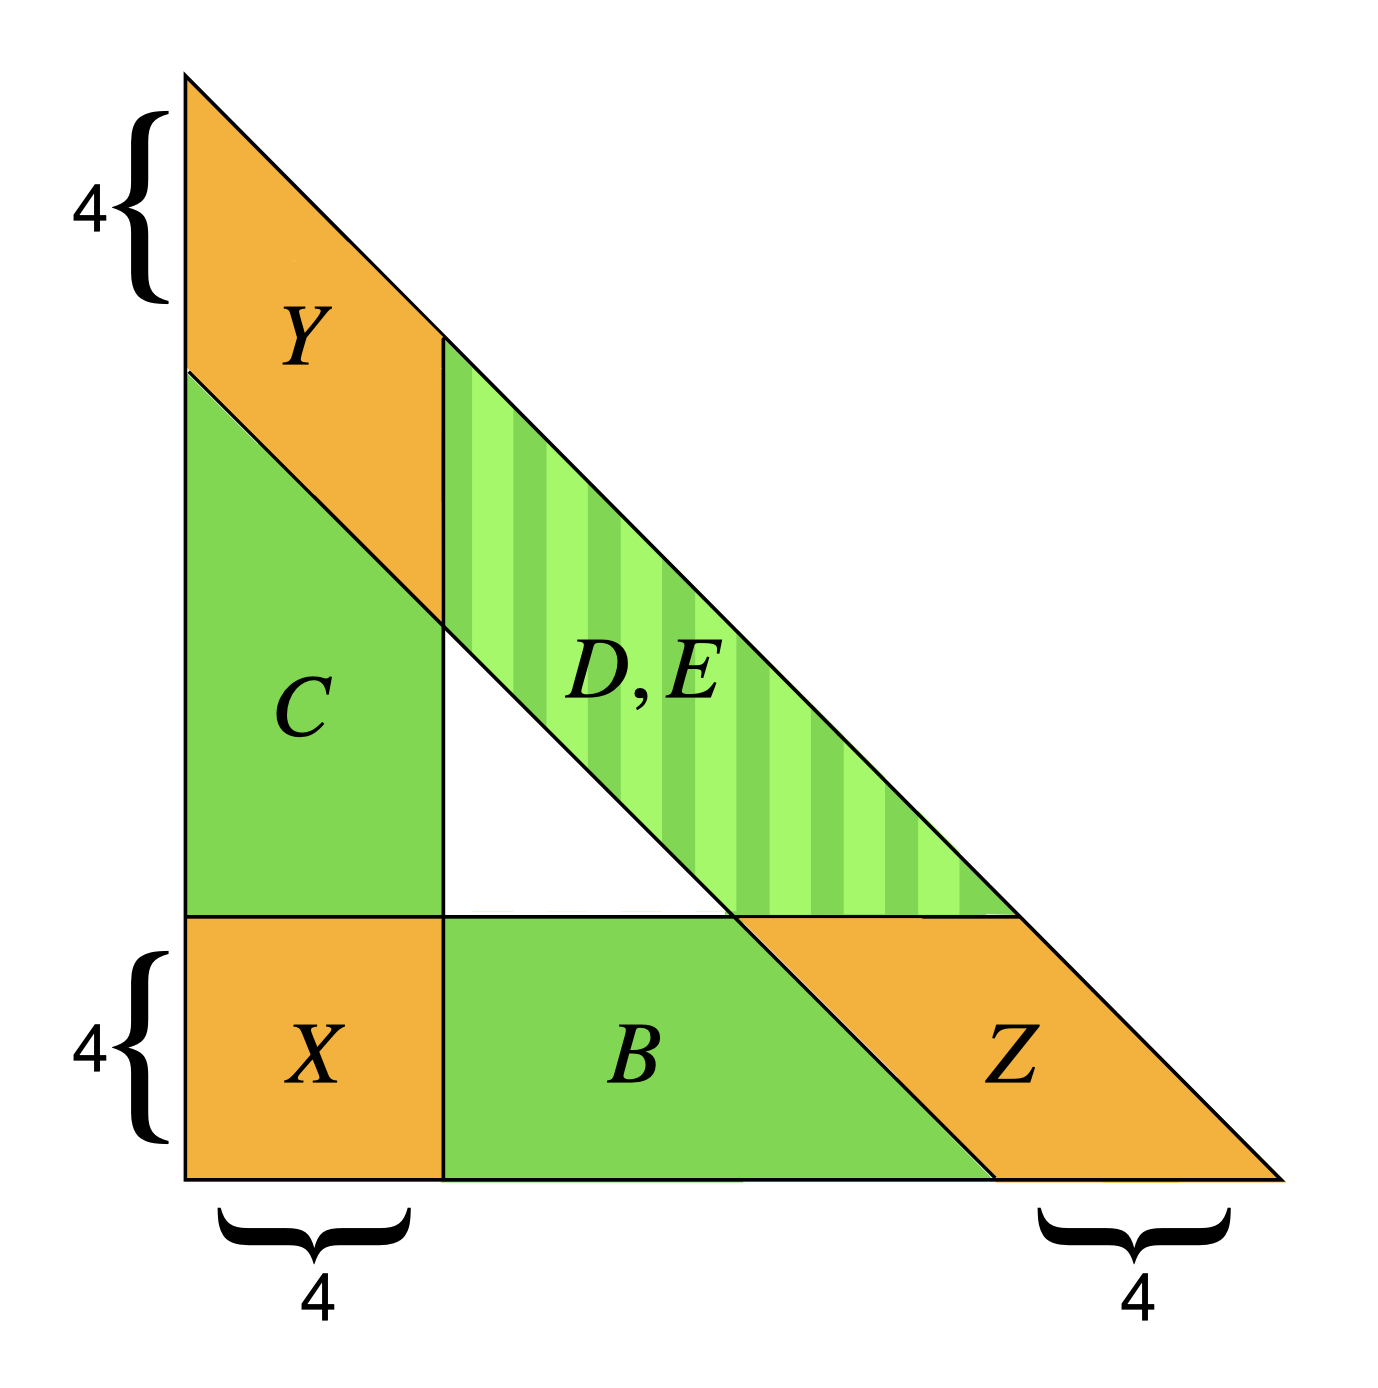
\includegraphics[width=0.75\textwidth]{assets/contactions-4.png}
    \caption{This figure illustrates the contraction variables and is taken from \cite{bik2022classifying}. The yellow areas \( X, Y, Z \) represent formal variables \( x_{i,j} \) that are unaffected by the contraction. The mint areas \( B, C, D \) represent rows and columns of vertices that are merged into a single vertex. The area \( D \) is further divided into areas \( D_1, D_2 \) by alternating columns.}
\end{figure}

\begin{definition}
Let \( x_{i,j} \) be formal variables indexed by \( V_d \). We merge a subset of rows and columns of formal variables \( x_{i,j} \) in \( V_d \) into a single vertex by defining the following \emph{contraction variables}:
\begin{align*}
    y_{i,j} &\coloneqq x_{i, d-3-i+j} \quad \text{ for } i,j = 0, \dots, 3, \\
    z_{i,j} &\coloneqq x_{d-3-j+i,j} \quad \text{ for } i,j = 0, \dots, 3, \\
    b_j &\coloneqq x_{4,j} + \dots + x_{d-4-j,j} \quad \text{ for } j = 0, \dots, 3, \\
    c_i &\coloneqq x_{i,4} + \dots + x_{i,d-4-i} \quad \text{ for } i = 0, \dots, 3, \\
    d_k &\coloneqq \begin{cases}
        x_{4,d-4-k} + x_{6,d-6-k} + \dots + x_{d-4-k,4} & \text{ if \( d + k \) is even} \\
        x_{4,d-4-k} + x_{6,d-6-k} + \dots + x_{d-5-k,5} & \text{ if \( d + k \) is odd}
    \end{cases} \quad \text{ for } k = 0, \dots, 3, \\
    e_k &\coloneqq \begin{cases}
        x_{5,d-5-k} + x_{7,d-7-k} + \dots + x_{d-5-k,5} & \text{ if \( d + k \) is even} \\
        x_{5,d-5-k} + x_{7,d-7-k} + \dots + x_{d-4-k,4} & \text{ if \( d + k \) is odd}
    \end{cases} \quad \text{ for } k = 0, \dots, 3.
\end{align*}
\end{definition}

Let us visualize the contraction variables for \( d = 16 \) in the following figure.

\begin{figure}[H]
    \begin{align*}
        \begin{array}{cccccccccccccccccccc}
            y_{0,3} & & & & & & & & & & & & \\
            y_{0,2} & y_{1,3} & & & & & & & & & & & \\
            y_{0,1} & y_{1,2} & y_{2,3} & & & & & & & & & & \\
            y_{0,0} & y_{1,1} & y_{2,2} & y_{3,3} & & & & & & & & & \\
            c_0 & y_{1,0} & y_{2,1} & y_{3,2} & d_0 & & & & & & & & \\
            c_0 & c_1 & y_{2,0} & y_{3,1} & d_1 & e_0 & & & & & & & \\
            c_0 & c_1 & c_2 & y_{3,0} & d_2 & e_1 & d_0 & & & & & & \\
            c_0 & c_1 & c_2 & c_3 & d_3 & e_2 & d_1 & e_0 & & & & & \\
            c_0 & c_1 & c_2 & c_3 &  *  & e_3 & d_2 & e_1 & d_0 & & & & \\
            c_0 & c_1 & c_2 & c_3 &  *  & * & d_3 & e_2 & d_1 & e_0 & & & \\
            c_0 & c_1 & c_2 & c_3 &  *  & * & * & e_3 & d_2 & e_1 & d_0 & & \\
            c_0 & c_1 & c_2 & c_3 &  *  & * & * & * & d_3 & e_2 & d_1 & e_0 & \\
            c_0 & c_1 & c_2 & c_3 &  *  & * & * & * & * & e_3 & d_2 & e_1 & d_0 \\
            x_{0,3} & x_{1,3} & x_{2,3} & x_{3,3} & b_3 & b_3 & b_3 & b_3 & b_3 & b_3 & z_{0,3} & z_{1,3} & z_{2,3} & z_{3,3} \\
            x_{0,2} & x_{1,2} & x_{2,2} & x_{3,2} & b_2 & b_2 & b_2 & b_2 & b_2 & b_2 & b_2 & z_{0,2} & z_{1,2} & z_{2,2} & z_{3,2} \\
            x_{0,1} & x_{1,1} & x_{2,1} & x_{3,1} & b_1 & b_1 & b_1 & b_1 & b_1 & b_1 & b_1 & b_1 & z_{0,1} & z_{1,1} & z_{2,1} & z_{3,1} \\
            x_{0,0} & x_{1,0} & x_{2,0} & x_{3,0} & b_0 & b_0 & b_0 & b_0 & b_0 & b_0 & b_0 & b_0 & b_0 & z_{0,0} & z_{1,0} & z_{2,0} & z_{3,0}
        \end{array}
    \end{align*}  
    \caption{Contraction variables for \( d = 16 \) are depicted.}
\end{figure}

As we can see, the vertices \( x_{0,4}, \dots, x_{0, d-4} \) are merged into the contraction variable \( c_0 \) by summing them up. Similarly, the formal variables \( x_{i,4}, \dots, x_{i,d-4-i} \) are merged into \( c_i \) for \( i = 1,2,3 \).

We remind that hyperfield Pascal forms are expressed as sums \( \sum_{(i,j) \in V_d} \lambda_{i,j} x_{i,j} \) with \( \lambda_{i,j} \in H \). The key insight is that there are some Pascal forms that can be expressed in terms of the contraction variables \( c_0 , c_1, c_2\) and \( c_3 \) instead of the original variables \( x_{i,j} \) for all vertices \( (i,j) \) in the \( C \)-area of Figure \ref{fig:contractions-42342432}.

\begin{example}
    Consider the Pascal form \( \mathrm{diag}(1) \) in \( \mathbb{Z}^{V_{16}} \). Its support is depicted in the following figure:
    \begin{verbatim}
        .
        +  +
        +  +  . 
        +  +  .  .  
        +  +  .  .  .  
        +  +  .  .  .  .  
        +  +  .  .  .  .  .  
        +  +  .  .  .  .  .  .  
        +  +  .  .  .  .  .  .  .
        +  +  .  .  .  .  .  .  .  .  
        +  +  .  .  .  .  .  .  .  .  .
        +  +  .  .  .  .  .  .  .  .  .  .
        +  +  .  .  .  .  .  .  .  .  .  .  .
        +  +  .  .  .  .  .  .  .  .  .  .  .  .
        +  +  .  .  .  .  .  .  .  .  .  .  .  .  .
        +  +  .  .  .  .  .  .  .  .  .  .  .  .  .  .
        +  +  .  .  .  .  .  .  .  .  .  .  .  .  .  .  .
    \end{verbatim}
    We see that \( \mathrm{diag}(1) = x_{0,0} + x_{0,1} + x_{0,2} + x_{0,3} + x_{1,0} + x_{1,1} + x_{1,2} + x_{1,3} + y_{0,0} + y_{0,1} + y_{0,2} + y_{1,0} + y_{1,1} + y_{1,2} + y_{1,3} + c_0 + c_1\).
\end{example}

The previous example also demonstrates the expression \( \mathrm{diag}(1) = x_{0,0} + x_{0,1} + x_{0,2} + x_{0,3} + x_{1,0} + x_{1,1} + x_{1,2} + x_{1,3} + y_{0,0} + y_{0,1} + y_{0,2} + y_{1,0} + y_{1,1} + y_{1,2} + y_{1,3} + c_0 + c_1 \) is \emph{independent} of the degree \( d \), i.e. if we were to consider the Pascal form \( \mathrm{diag}(1) \) in \( \mathbb{Z}^{V_{d}} \) for some arbitrary \( d \), the expression would still hold. This is great news since it allows us to express Pascal forms in terms of contraction variables for all degrees \( d \) at once.

So far, we have only considered the contraction variables \( c_0, c_1, c_2 \), and \( c_3 \). As we might expect, we can also express some Pascal forms in terms of the contraction variables \( b_0, b_1, b_2, b_3 \), \( d_0, d_1, d_2, d_3 \), \( e_0, e_1, e_2, e_3 \), \( y_{i,j} \), and \( z_{i,j} \). We will now find these kinds of Pascal forms that can be represented in terms of the contraction variables independent of the degree \( d \).